\chapter{El projecte Quadriga}

El projecte, amb el codi font i alguns exemples, es pot trobar a la pàgina \url{http://quadriga.googlecode.com}. Addicionalment també es pot trobar aquesta mateixa memòria. En el moment d'escriure aquesta memòria, el projecte es pot aconseguir d'un servidor de {\bf Subversion}, actualment a la revisió número 100. El codi està pensat per a ser compilat amb la {\em IDE Eclipse} de la següent manera:

\begin{enumerate}
  \item Cal instal·lar Eclipse amb els plugins {\em subclipse} \url{http://subclipse.tigris.org/} i {\em JavaCC Eclipse Plug-in} \url{http://eclipse-javacc.sourceforge.net/}.
  
  \item Cal descarregar el projecte {\bf SVN} des d'Eclipse amb repositori a \url{http://quadriga.googlecode.com/svn/trunk/Quadriga Parser/}. \\
        Alternativament es pot descarregar tot el projecte amb {\bf SVN} ja sigui amb la consola o usant un programa com {\bf Tortoise SVN} \url{http://tortoisesvn.tigris.org/}.
        
  \item Descarregar les llibreries {\bf LWJGL} \url{http://lwjgl.org/download.php} i {\bf HSQLDB} \url{http://sourceforge.net/projects/hsqldb/files/}. 
        Incloure ambdues llibreries al projecte d'Eclipse (figura \ref{fig:incloure}).
        
  \item Finalment cal indicar-li a l'Eclipse on troba les llibreries dinàmiques de {\bf LWJGL} (figura \ref{fig:incloure3}).
\end{enumerate}

\begin{figure}
  \centering
  \subfloat[Obrir les propietats del projecte]{\label{fig:incloure1}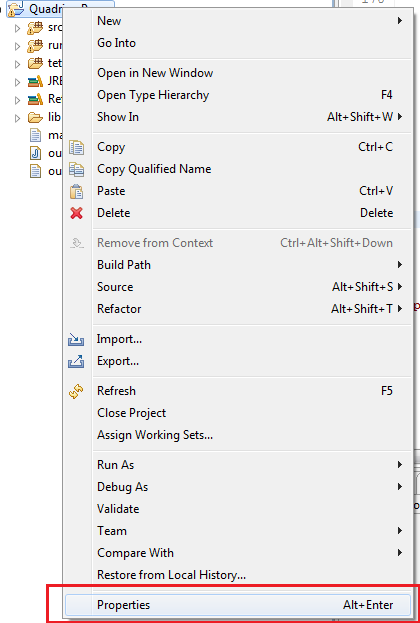
\includegraphics[width=0.48\textwidth]{./img/incloure1.png}}                
  \subfloat[Afegir els les llibreries (jar) necessàries]{\label{fig:incloure2}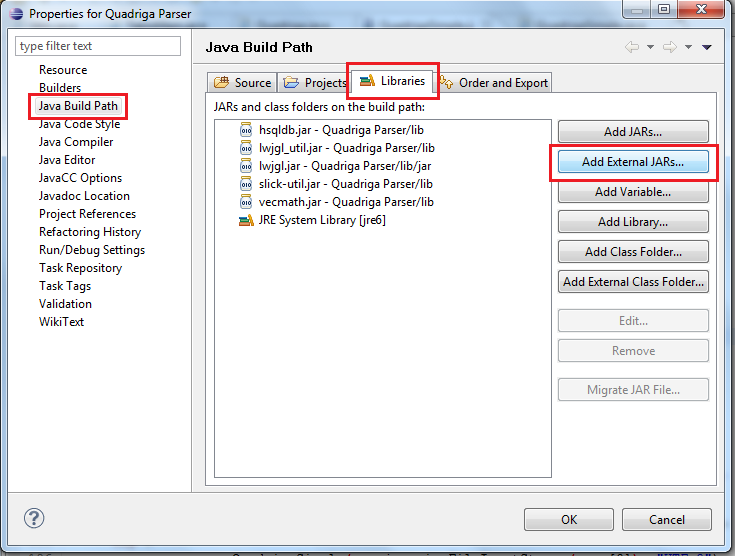
\includegraphics[width=0.48\textwidth]{./img/incloure2.png}}
  \caption{Com incloure les llibreries necessàries}
  \label{fig:incloure}
\end{figure}

\begin{figure}
  \centering
  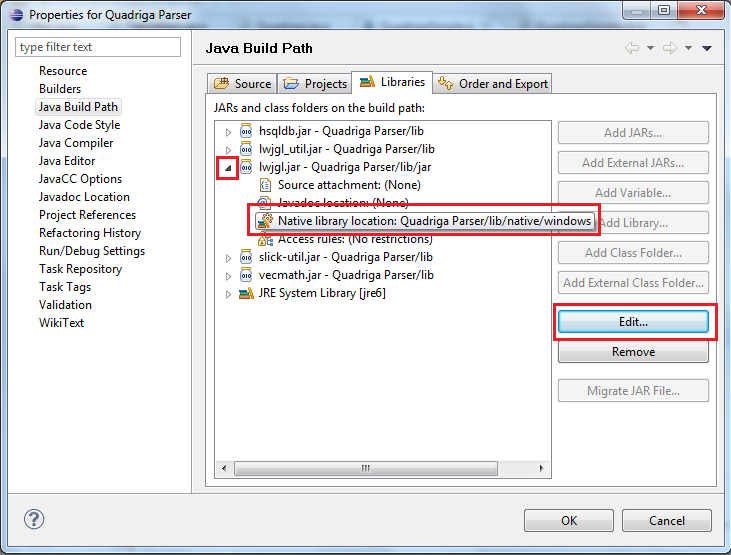
\includegraphics[width=0.58\linewidth]{./img/incloure3.png}
  \caption{Indicar-li el path a les llibreries dinàmiques \label{fig:incloure3}}
\end{figure}